\documentclass[11pt]{article}
\usepackage[margin=1in]{geometry}
\usepackage{amsmath,amssymb,graphicx,booktabs,hyperref,float}
\setlength{\parskip}{0.4em}
\setlength{\parindent}{0pt}

\title{Data 37711: Homework 2}
\author{Zien Guo}
\date{}

\begin{document}
\maketitle

\noindent\textbf{Code:} \url{https://github.com/zienguo-SilverHand/DATA37711} (directory \texttt{homework\_2}; run \texttt{pip install -r requirements.txt \&\& bash run\_all.sh}). Notebooks \texttt{hw2\_q1}, \texttt{hw2\_q2}, \texttt{hw2\_q3} correspond to Problems 1--3.

%------------------------------------------------------------
\section*{Problem 1}

\paragraph{(a)}
Let $g(x)=(g_1(x),g_2(x))$. Take
\[
f_\mu(x)=g_1(x),\qquad f_\sigma(x)=\log\!\big(1+e^{g_2(x)}\big).
\]
The mean is unconstrained, while the softplus maps $\mathbb{R}\to(0,\infty)$, so $f_\sigma>0$.

\paragraph{(b)}
With $Y\mid X\sim\mathcal{N}(f_\mu(X),f_\sigma(X)^2)$, the density of one observation is
\[
p(y\mid x)=\frac{1}{\sqrt{2\pi}\,f_\sigma(x)}\exp\!\left(-\frac{(y-f_\mu(x))^2}{2f_\sigma(x)^2}\right).
\]
Maximum likelihood chooses $\theta$ to maximize $\prod_{i=1}^n p(y_i\mid x_i)$, which is equivalent to maximizing $\sum_i\log p(y_i\mid x_i)$, or minimizing the negative log-likelihood:
\[
-\sum_{i=1}^n\log p(y_i\mid x_i)=\sum_{i=1}^n\left[\frac{(y_i-f_\mu(x_i))^2}{2f_\sigma(x_i)^2}+\log f_\sigma(x_i)+\tfrac12\log 2\pi\right].
\]
Dropping the constant and averaging gives the loss
\[
\mathcal{L}(\theta)=\frac1n\sum_{i=1}^n\left[\frac{(y_i-f_\mu(x_i))^2}{2f_\sigma(x_i)^2}+\log f_\sigma(x_i)\right].
\]

\paragraph{(c)}
This part is implemented in \texttt{hw2\_q1.ipynb} (70/15/15 train/validation/test split, MLP with early stopping on validation loss). Baselines are the training mean, linear regression and gradient boosting (scikit-learn); each is paired with a Gaussian with constant $\sigma$ equal to its training residual standard deviation to compute NLL. Test results:

\begin{table}[H]
\centering
\begin{tabular}{lccc}
\toprule
Model & RMSE (min) & MAE (min) & NLL \\
\midrule
Mean & 7.688 & 5.664 & 3.459 \\
Linear regression & 7.473 & 5.554 & 3.430 \\
Gradient boosting & 4.285 & 2.982 & 2.874 \\
Gaussian MLP & \textbf{3.898} & \textbf{2.454} & \textbf{2.621} \\
\bottomrule
\end{tabular}
\end{table}
The MLP beats all baselines on every metric.

\paragraph{(d)}
For an input $x$, let $\hat\mu(x)=f_{\hat\mu}(x)$ and $\hat\sigma(x)=f_{\hat\sigma}(x)$ be the fitted model's outputs. Then $Y\mid x\sim\mathcal{N}(\hat\mu(x),\hat\sigma(x)^2)$ and
\[
\hat P(Y<45\mid x)=P\!\left(\frac{Y-\hat\mu(x)}{\hat\sigma(x)}<\frac{45-\hat\mu(x)}{\hat\sigma(x)}\right)=\Phi\!\left(\frac{45-\hat\mu(x)}{\hat\sigma(x)}\right),
\]
where $\Phi$ is the standard normal CDF.

\paragraph{(e)}
I computed $\hat p_i=\Phi\big((45-\hat\mu(x_i))/\hat\sigma(x_i)\big)$ on the test set and compared with $\mathbf 1\{y_i<45\}$. For accuracy, I threshold $\hat p_i$ at 0.5. The baselines use the same formula with their constant $\sigma$.

\begin{table}[H]
\centering
\begin{tabular}{lccc}
\toprule
Model & Brier score & Log-loss & Accuracy \\
\midrule
Mean & 0.0043 & 0.0532 & 0.9957 \\
Linear regression & 0.0043 & 0.0445 & 0.9957 \\
Gradient boosting & 0.0031 & 0.0318 & \textbf{0.9967} \\
Gaussian MLP & \textbf{0.0030} & \textbf{0.0213} & 0.9965 \\
\bottomrule
\end{tabular}
\end{table}
Since 99.57\% of test trips are under 45 minutes (only 0.43\% take 45 minutes or longer), predicting ``under 45'' for every trip already gives accuracy 0.9957, so accuracy barely separates the models. The MLP has the best Brier score and log-loss.

%------------------------------------------------------------
\section*{Problem 2}

\paragraph{(a)}
\texttt{StockCode} has 3{,}665 unique values and \texttt{CustomerID} has 4{,}339, so one-hot encoding needs 8{,}004 columns for 397{,}924 rows. It is possible to store sparsely, but the input is very high-dimensional and many categories are rare, so target encoding or embeddings are better choices. \texttt{Quantity} is heavy-tailed (median 6, maximum 80{,}995), so I model $\log(1+\texttt{Quantity})$ with MSE. The data is split 70/15/15\% (validation used for early stopping). All errors below are on the $\log(1+\cdot)$ scale.

\paragraph{(b)--(d)}
Implemented in \texttt{hw2\_q2.ipynb}. All three models use the same MLP (two hidden layers of 128) and differ only in inputs: (b) the two target-encoded features (scikit-learn \texttt{TargetEncoder}; training-set encodings use its 5-fold cross-fitted \texttt{fit\_transform}, so a row's own label does not enter its encoding, and validation/test rows use the encoder fit on the full training set); (c) a 16-dimensional embedding for each feature; (d) both. Test results:

\begin{table}[H]
\centering
\begin{tabular}{lcc}
\toprule
Model & Test RMSE & Test MAE \\
\midrule
Mean baseline & 1.0072 & 0.8193 \\
(b) Target encoding & 0.5797 & 0.4263 \\
(c) Embeddings & 0.5474 & 0.3905 \\
(d) Target encoding + embeddings & \textbf{0.5369} & \textbf{0.3799} \\
\bottomrule
\end{tabular}
\end{table}
Embeddings beat target encoding, and combining the two is slightly better again.

\paragraph{(e)}
Target encoding compresses each category into a single number (its mean target), which is noisy for rare categories and ignores the other feature. An embedding layer learns a vector per category jointly with the network, so it can store whatever helps prediction, and the network can combine the \texttt{StockCode} and \texttt{CustomerID} vectors nonlinearly to capture product--customer interactions. This is consistent with the test results above. The combined model adds a small gain, presumably because the target-encoded values give a useful summary for rare categories. Almost all test rows (59{,}635 of 59{,}689) have both categories seen in training; the few rows with unseen categories (30 and 24) are too few to draw conclusions.

%------------------------------------------------------------
\section*{Problem 3}

\paragraph{(a)}
Figure~\ref{fig:data} shows the training data. The response is smooth and nonlinear: lowest (about $-1$) near $(x_1,x_2)\approx(-1.5,0)$, and highest (about 5) near the top and bottom edges at $x_1\approx1$ to $2$, like a noisy saddle.

\begin{figure}[H]
\centering
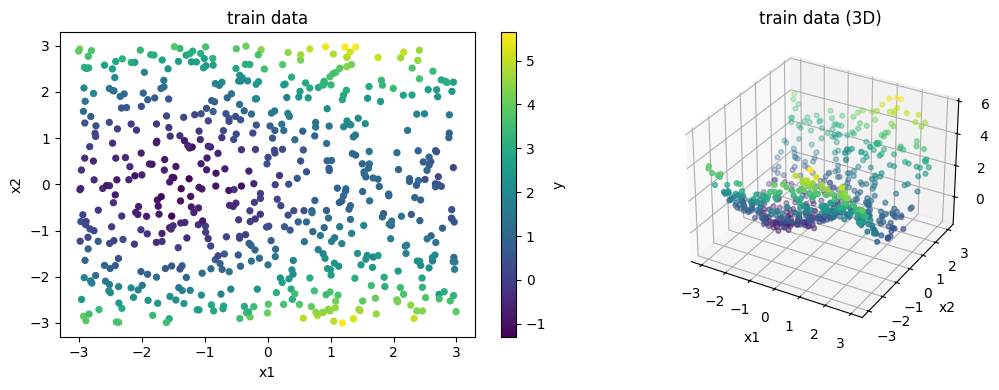
\includegraphics[width=0.85\textwidth]{figures/q3_1.png}
\caption{Training data.}\label{fig:data}
\end{figure}

\paragraph{(b)}
RKS with $D=500$ sine/cosine features and ridge penalty $\lambda=10^{-3}$ (fixed); I swept $\sigma$ over 20 log-spaced values in $[10^{-1.5},10]$ (Figure~\ref{fig:rks}). Small $\sigma$ (high-frequency features) overfits badly, while for $\sigma\gtrsim0.3$ the validation MSE is flat and small. The best value is $\sigma=5.46$ (validation MSE $0.0362$).

\begin{figure}[H]
\centering
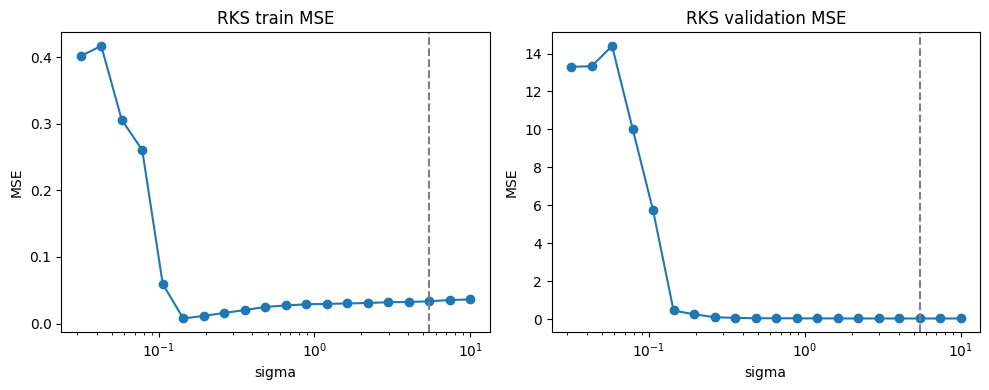
\includegraphics[width=0.8\textwidth]{figures/q3_2.png}
\caption{RKS training (left) and validation (right) MSE vs.\ $\sigma$; dashed line is the best $\sigma$.}\label{fig:rks}
\end{figure}

\paragraph{(c)}
One-hidden-layer ReLU MLP (Adam, lr $10^{-2}$, batch 64, 300 epochs); I swept the hidden dimension over $\{2,\dots,512\}$ (Figure~\ref{fig:mlp}). Widths 2 and 4 underfit; the best is 64 (validation MSE $0.0403$), and the widest networks are slightly worse.

\begin{figure}[H]
\centering
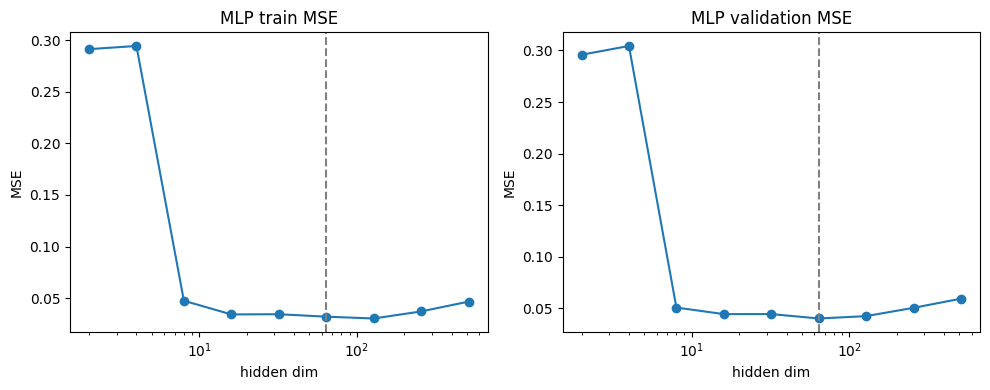
\includegraphics[width=0.8\textwidth]{figures/q3_3.png}
\caption{MLP training (left) and validation (right) MSE vs.\ hidden dimension.}\label{fig:mlp}
\end{figure}

\paragraph{(d)}
After refitting on the training set only (same seeds, so the validation MSEs equal the sweep values) with the selected hyperparameters, the validation MSE is $0.0362$ for RKS and $0.0403$ for the MLP. RKS is slightly better, but the gap is small and comes from a single seed, so I do not claim a clear winner. The test predictions are in \texttt{rks\_test\_predictions.csv} and \texttt{mlp\_test\_predictions.csv}.

Figure~\ref{fig:surf} compares the fitted surfaces with the data. Both capture the basin near $(-1.5,0)$ and the high regions at the top and bottom edges. The RKS surface is smoother, while the MLP surface shows slight straight-edged facets because a ReLU network is piecewise linear.

\begin{figure}[H]
\centering
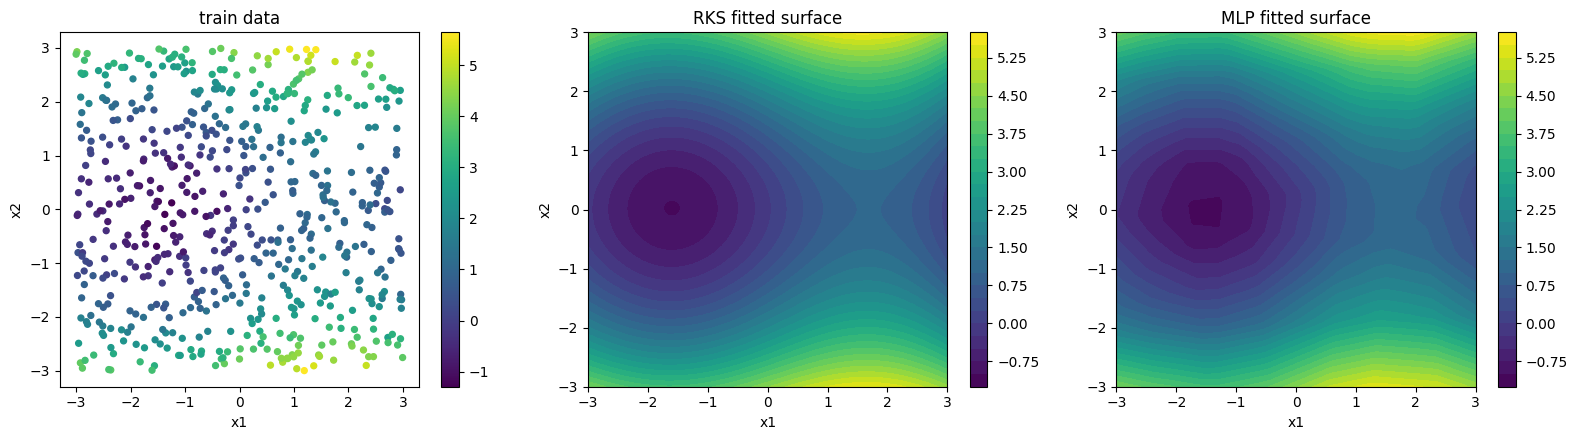
\includegraphics[width=\textwidth]{figures/q3_4.png}
\caption{Training data (left), RKS surface (middle), MLP surface (right).}\label{fig:surf}
\end{figure}

\end{document}
